%%%%%%%%%%%%%%%%%%%%%%%%%%%%%%%%%%%%%%%%%
% Simple Sectioned Essay Template
% LaTeX Template
%
% This template has been downloaded from:
% http://www.latextemplates.com
%
% Note:
% The \lipsum[#] commands throughout this template generate dummy text
% to fill the template out. These commands should all be removed when 
% writing essay content.
%
%%%%%%%%%%%%%%%%%%%%%%%%%%%%%%%%%%%%%%%%%

%----------------------------------------------------------------------------------------
%	PACKAGES AND OTHER DOCUMENT CONFIGURATIONS
%----------------------------------------------------------------------------------------

\documentclass[12pt]{article} % Default font size is 12pt, it can be changed here

\usepackage[brazil]{babel}
\usepackage[utf8]{inputenc}
\usepackage{geometry} % Required to change the page size to A4
\geometry{a4paper} % Set the page size to be A4 as opposed to the default US Letter

\usepackage{graphicx} % Required for including pictures

\usepackage{float} % Allows putting an [H] in \begin{figure} to specify the exact location of the figure
\usepackage{wrapfig} % Allows in-line images such as the example fish picture

\usepackage{lipsum} % Used for inserting dummy 'Lorem ipsum' text into the template

\linespread{1.2} % Line spacing

%\setlength\parindent{0pt} % Uncomment to remove all indentation from paragraphs

\graphicspath{{Pictures/}} % Specifies the directory where pictures are stored

\begin{document}

%----------------------------------------------------------------------------------------
%	TITLE PAGE
%----------------------------------------------------------------------------------------

\begin{titlepage}

\newcommand{\HRule}{\rule{\linewidth}{0.5mm}} % Defines a new command for the horizontal lines, change thickness here

\center % Center everything on the page

\textsc{\LARGE Universidade Federal de Pelotas}\\[1.5cm] % Name of your university/college
%\textsc{\Large Keeping a Beat on the Heart}\\[0.5cm] % Major heading such as course name
%\textsc{\large Arrhythmia Monitoring System (AMS)}\\[0.5cm] % Minor heading such as course title

\HRule \\[0.4cm]
{ \huge \bfseries Arrhythmia Monitoring System (AMS)}\\[0.4cm] % Title of your document
\HRule \\[1.5cm]

\begin{minipage}{0.4\textwidth}
\begin{flushleft} \large
\emph{Author:}\\
Alexandre Costa % Your name
\end{flushleft}
\end{minipage}

\vfill % Fill the rest of the page with whitespace

\end{titlepage}

%----------------------------------------------------------------------------------------
%	TABLE OF CONTENTS
%----------------------------------------------------------------------------------------

\tableofcontents % Include a table of contents

\newpage % Begins the essay on a new page instead of on the same page as the table of contents 

%----------------------------------------------------------------------------------------
%	ABISTRACT
%----------------------------------------------------------------------------------------

\section{Abstract} % Major section

In the scope of ubiquitous computing, one of the key issues is the awareness of context, which includes diverse aspects of the user’s situation including his activities, physical surroundings, location, emotions and social relations, device and network characteristics and their interaction with each other. This contextual knowledge is typically acquired from physical, virtual or logical sensors. To overcome problems of heterogeneity and hide complexity, a significant number of middleware approaches have been proposed for systematic and coherent access to manifold context parameters. These frameworks deal particularly with context representation, context management and reasoning, i.e. deriving abstract knowledge from raw sensor data. This article surveys not only related work in these three categories but also the required evaluation principles.

Index Terms—Middleware, Context Provisioning, Context Management, Context Representation, Evaluation, Simulation, Ubiquitous Computing.


%----------------------------------------------------------------------------------------
%	RESUMO
%----------------------------------------------------------------------------------------

\section{Resumo} % Major section

No âmbito da computação ubíqua, uma das questões-chaves é a consciência do contexto, que inclui diversos aspectos da situação do usuário, incluindo suas atividades, ambiente físico, localização, emoções e relações sociais, dispositivos e características da rede e sua interação uns com os outros . Este conhecimento contextual é geralmente adquirido a partir de sensores físicos, virtuais ou lógica. Para superar os problemas de heterogeneidade e de complexidade ocultar, um número significativo de abordagens de middleware têm sido propostos para o acesso sistemática e coerente com os parâmetros de contexto múltiplas. Estes quadros lidar especialmente com a representação contexto, gerenciamento de contexto e de raciocínio, ou seja, decorrentes do conhecimento abstrato a partir dos dados brutos do sensor. Este artigo examina não só o trabalho relacionado nestas três categorias, mas também os princípios de avaliação necessários.

Palavras-chave: Middleware, Provisioning contexto, gestão de contexto, representação, avaliação, simulação de contexto, Computação Ubíqua.

%----------------------------------------------------------------------------------------
%	INTRODUÇÃO
%----------------------------------------------------------------------------------------

\section{Introdução} % Major section

%Ubiquitous Computing (UbiComp) paraphrases the paradigm of hardware and software components being transparently interwoven by means of wireless communication. Value added computer intelligence resulting from the smart and autonomous networking of multiple devices has much more potential than that originating from a single, isolated device. A key objective of these systems is to significantly simplify Human Computer Interaction (HCI) by deploying sensors, processors and actuators in the fabric of everyday life, such that their presence and complexity is hidden from users [1]. UbiComp is commonly understood as the next wave of an evolution chain of computing paradigms, which have gone through the personal computing (second generation) and distributed computing (third generation) from the roots of mainframe computing. Figure 1 illustrates our view of this evolution and highlights some of the features pertinent to the realisation of UbiComp.

Ubiquitous Computing (UbiComp) parafraseia o paradigma de componentes de software que está sendo transparente interligados por meio de comunicação sem fio e hardware. Valor acrescentado inteligência computacional resultante da rede inteligente e autônoma de vários dispositivos tem muito mais potencial do que o proveniente de um único dispositivo, isolado. Um dos principais objetivos destes sistemas é o de simplificar significativamente Interação Humano-Computador (IHC), implantando sensores, processadores e atuadores no tecido da vida cotidiana, de modo que a sua presença e complexidade está escondida dos usuários [1]. UbiComp é comumente entendido como a próxima onda de uma cadeia de evolução dos paradigmas de computação, que passaram a computação pessoal (segunda geração) e computação distribuída (terceira geração) a partir das raízes da computação em mainframe. A figura 1 ilustra a nossa visão dessa evolução e destaca algumas das características pertinentes para a realização de UbiComp.

%------------------------------------------------

\subsection{Context and Context-awareness} % Sub-section

%Context is information about a location, its environmental attributes (e.g. noise level, light intensity, temperature, and motion) and the people, devices, objects and software agents that it contains. Context may also include system capabilities, services offered and sought, the activities and tasks in which people and computing entities are engaged, and their situational roles, beliefs, and intentions. Context-awareness is one of the key enablers to facilitate proactive support of users in their current situation. Users do not have to define their situation explicitly by utilising time consuming and counter-intuitive input devices but it is implicitly recognised by the “smart” environment instead. The idea that computing devices can sense and react to stimuli from users’ environment is labelled as context-aware computing.

Contexto é a informação sobre a localização, os seus atributos ambientais (por exemplo, nível de ruído, intensidade de luz, temperatura e movimento) e as pessoas, aparelhos, objetos e agentes de software que contém. Contexto também pode incluir sistema capacidades, serviços oferecidos e procurados, as atividades e tarefas em que as pessoas e entidades de computação estão envolvidos, e seus papéis situacionais, crenças e intenções. Context-awareness é um dos elementos fundamentais para facilitar o apoio pró-ativa de usuários em sua situação atual. O usuário não tem que definir sua situação explicitamente utilizando demorado e dispositivos de entrada de contra-intuitivos, mas é implicitamente reconhecida pelo ambiente "inteligente" em seu lugar. A idéia de que os dispositivos de computação pode sentir e reagir aos estímulos do ambiente dos usuários é rotulado como a computação context-aware.

\begin{figure}[H]
\center{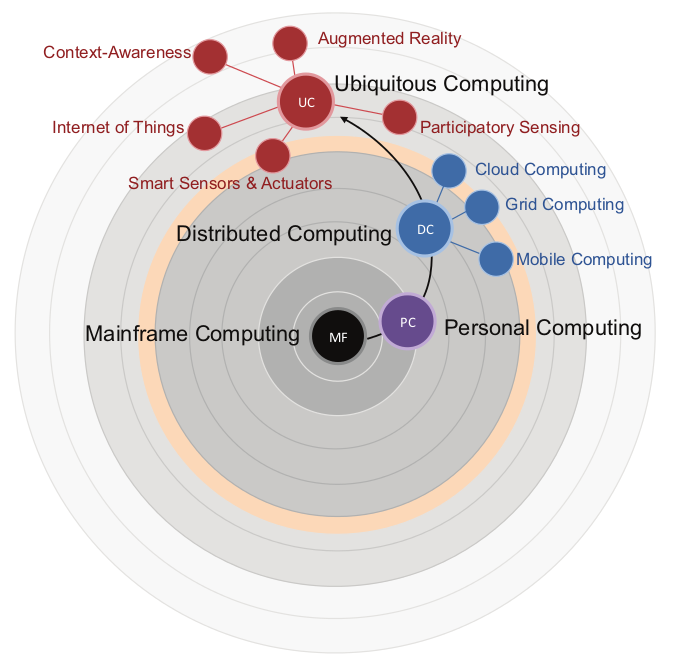
\includegraphics[width=0.5\linewidth]{figura1}}
\caption{Evolution Chain and Features of Ubiquitous Computing}
\label{fig:speciation}
\end{figure}

%User identity and location are the most prominent context parameters widely utilised in various location-based services. Beyond that, as defined by Dey [2], context may comprise any information relevant for describing the users’ interaction with each other and with context-aware services and applications. In our digital world there is a large amount of distributed information available describing such interaction in a diverse way, e.g. the location of a person (GPS enabled smart phones), activity (phone-based gyroscope, accelerometer, foreground applications, digital calendar), social situation (location, time of the day, proximity to friends) and evolving preferences (self-configured and history-based digital profiles).

Identidade do usuário ea localização são os parâmetros de contexto mais proeminentes amplamente utilizados em vários serviços baseados em localização. Além disso, tal como definido por Dey [2], o contexto pode compreender todas as informações pertinentes para descrever a interacção dos utilizadores uns com os outros e com os serviços sensíveis ao contexto e aplicações. Em nosso mundo digital, há uma grande quantidade de informação distribuída disponível descrevendo essa interação de forma diversa, por exemplo, a localização de uma pessoa (GPS habilitado telefones inteligentes), atividade (giroscópio por telefone, acelerômetro, aplicativos em primeiro plano, calendário digital), situação social (localização, hora do dia, a proximidade com os amigos) e as preferências em evolução (auto-configurado e história com base em perfis digitais).

%Context-awareness is an interdisciplinary field of research involving communication engineering and computer science, more precisely mobile communication, HCI (Human Computer Interaction) design, sensor data processing, feature extraction and artificial intelligence. In these communities a large set of application domains benefiting from contextual awareness has been proposed. Use cases of high potential include health care and well-being [3], e-learning and campus life [4], tourism and travelling [5], office and other business applications [6], advertising and e-commerce [7], entertainment [8], gaming [9] and social community applications [10]. Moreover, smart places – an emerging research field in itself – heavily rely on context-awareness. A smart place is a geographically bounded area providing smart interaction between computational devices and users located in the space. Smart offices, smart labs and smart homes are examples of smart places [11].

Context-awareness é um campo interdisciplinar de pesquisa envolvendo inteligência artificial engenharia de comunicação e ciência da computação, comunicação, mais precisamente móvel, projeto HCI (Human Computer Interaction), processamento de dados do sensor, extração de características e. Nessas comunidades, foi proposto um grande conjunto de domínios de aplicações que beneficiam de consciência contextual. Os casos de uso de alto potencial incluem cuidados de saúde e bem-estar [3], e-learning e de vida no campus [4], turismo e viajar [5], Office e outros aplicativos de negócios [6], publicidade e e-commerce [7] , entretenimento [8], o jogo [9] e aplicações sociais da comunidade [10]. Além disso, lugares inteligentes - um campo de pesquisa emergente em si - dependem fortemente do contexto consciência. Um lugar inteligente é uma área geograficamente delimitada proporcionando interação inteligente entre dispositivos computacionais e utilizadores situados no espaço. Escritórios inteligentes, laboratórios inteligentes e casas inteligentes são exemplos de lugares inteligentes [11].

%------------------------------------------------

\subsection{Context-aware Systems} % Sub-section

%The computing systems that are designed to provide context-aware services have to perform a variety of distinct functions. These include collection of raw data about the users and their environment, applying different reasoning techniques on such data to synthesise higher-level context information, storage of the context information in a retrievable and indexed format to make available when required, management and coordination of context and related information between different components of the systems, and to provide a platform for building, hosting or enabling context-aware applications and services.

Os sistemas de computação que são projetados para fornecer serviços sensíveis ao contexto têm que executar uma variedade de funções distintas. Estes incluem a coleta de dados brutos sobre os usuários e seu ambiente, aplicando diferentes técnicas de raciocínio em tais dados para sintetizar informações de contexto de nível superior, o armazenamento das informações de contexto em um formato recuperável e indexada a disponibilizar, quando necessário, gestão e coordenação de contexto e informações relacionadas entre os diferentes componentes dos sistemas, e para fornecer uma plataforma para a construção, hospedagem ou permitindo que aplicativos e serviços sensíveis ao contexto.

%A number of design approaches have been attempted for collective provisioning of these functions with the overall aim of making context information available about anything, any time, and anywhere. Context-aware systems are usually designed as middleware adopting a layered design – each functional layer hiding the details of the underlying layers (see Fig. 2). The primary benefit of this approach is the encapsulation of varying complexities of different functions. Each layer builds on the information made available by the layer below it, e.g. the Context Processing Layer uses data collected at the Data Acquisition Layer while the Applications Layer interacts with the Context Processing Layer to retrieve context and does not concern itself with the details of data acquisition or synthesis process.

Uma série de abordagens de design têm sido tentadas para provisionamento coletivas destas funções com o objectivo global de tornar a informação de contexto disponível sobre qualquer coisa, a qualquer hora e em qualquer lugar. Sistemas sensíveis ao contexto são normalmente concebidos como a adopção de middleware um projeto em camadas - cada camada funcional ocultando os detalhes das camadas subjacentes (ver Fig. 2.). A principal vantagem desta abordagem é a encapsulação de complexidades variando de diferentes funções. Cada camada baseia-se na informação disponibilizada pela camada abaixo dela, por exemplo, a camada de processamento Context usa dados coletados na camada de aquisição de dados, enquanto a camada de aplicações interage com a camada de processamento de contexto para recuperar contexto e não se preocupa com os detalhes do processo de aquisição ou a síntese de dados.

\begin{figure}[H]
\center{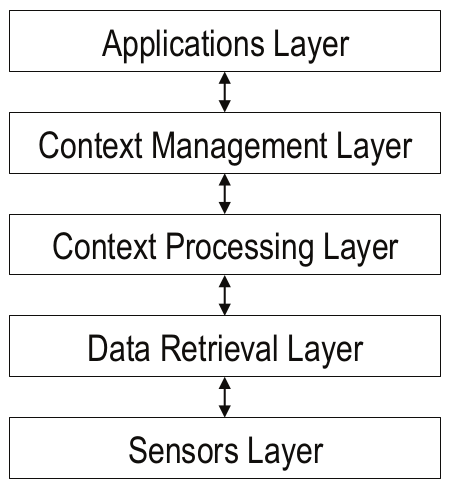
\includegraphics[width=0.5\linewidth]{figura2}}
\caption{Layered design of a context-aware middleware}
\label{fig:speciation}
\end{figure}

%With such a variety of functions to perform, the design, development, operation and evaluation of context-aware systems becomes a very complex task. Each functional layer in the middleware faces multidimensional challenges in contributing to the overall objective of context provisioning, e.g. with respect to data acquisition, to fully exploit awareness, context has to be acquired from heterogeneous sources, be processed and aggregated, as well as associated to users, devices and smart artefacts. Context is not only fetched from physical sensors but also from virtual and logical sensors, e.g. from databases or web services. This diversity and general applicability of context-awareness substantiate the need for architectural and functional support of ubiquitous services.

Com uma tal variedade de funções para executar, o design, desenvolvimento, operação e avaliação de sistemas sensíveis ao contexto torna-se uma tarefa muito complexa. Cada camada funcional no middleware enfrenta desafios multidimensionais em contribuir para o objectivo geral de abastecimento de contexto, por exemplo, no que diz respeito à aquisição de dados, para explorar plenamente consciência, o contexto tem de ser adquirido a partir de fontes heterogêneas, ser processado e agregados, bem como associados a usuários, dispositivos e artefatos inteligentes. Contexto não só é obtido a partir de sensores físicos, mas também a partir de sensores virtuais e lógico, por exemplo, de bancos de dados e serviços da web. Esta diversidade e aplicabilidade geral do contexto consciência fundamentar a necessidade de apoio arquitetônico e funcional dos serviços ubíquos.

%The design and operation of a context provisioning middleware is also laterally affected by the context model or representation scheme as it can influence the expressiveness and utility of the contextual information. In addition, current trends and innovations facilitate rapid development and deployment of new (smartphone) applications and services through the use of Service Creation Environments and specific Software Development Kits (SDK). Their context demands are unexpected and not easily predictable. The support of both existing context-aware applications/services and those emerging in the future requires functional scalability and gradual extendibility of the middleware with regard to new context types and new context processing capabilities. With their increasing processing, storage and communication capabilities, smartphones can be considered as personalised companions for interfacing with the digital world. Focussing on them as the main source of interaction allows for increasing the physical size of smart spaces to urban or even global extent. Therefore physical scalability is another prerequisite of a context provisioning middleware.

A concepção e operação de um contexto provisionamento middleware também é lateralmente afetado pelo modelo de contexto ou esquema de representação , uma vez que pode influenciar a expressividade ea utilidade da informação contextual. Além disso, as tendências e inovações atuais facilitar o rápido desenvolvimento e implementação de novas aplicações e serviços ( smartphone) com o uso de ambientes de criação de serviços e kits de desenvolvimento de software específicos ( SDK). Suas demandas de contexto são inesperados e não é facilmente previsível. O apoio de ambas as aplicações sensíveis ao contexto / serviços e os emergentes no futuro existentes requer escalabilidade funcional e capacidade de extensão gradual do middleware no que diz respeito a novos tipos de contexto e novas capacidades de processamento de contexto. Com os recursos de seu processamento aumentando, armazenamento e comunicação , os smartphones podem ser considerados como companheiros personalizados para a interface com o mundo digital. Centrando-se sobre eles como a principal fonte de interação permite aumentar o tamanho físico dos espaços inteligentes para extensão urbana ou mesmo global. Escalabilidade Portanto física é outro pré-requisito de um middleware de provisionamento contexto.

%The complex operation of a context-aware system is illustrated as an autonomic communication cycle in Fig. 3. The cycle highlights the acquisition of raw data from sensors and user profiles, undergoing an aggregation/processing stage through application of various reasoning mechanisms, the resultant information providing a basis for decision making, which can support adaptation in context-based services and eventually serve as an input to the next cycle of (higher-level) context generation. In general, decision and adaptation are considered to be rather application/service specific and therefore tend to be realised by the actual service application logic. The collection of sensor data and its analysis can be performed by a common middleware that is able to support a huge variety of application/service domains. Individual functions can be logically organised in different layers (cf. Fig.2) of the context-aware middleware. The middleware as a whole thus acts a glue that binds these functions together to achieve the goal of context-provisioning. The role of a context-aware middleware is therefore both central and critical to the effectiveness of context-aware services in the realm of ubiquitous computing, without which the virtual and real worlds can not be bridged.

A operação de um sistema complexo de reconhecimento de contexto é ilustrada como um ciclo de comunicação autonômica na FIG. 3. O ciclo destaca a aquisição de dados brutos de sensores e perfis de usuários , passando por uma fase de agregação / processamento através da aplicação de diversos mecanismos de raciocínio , a informação resultante fornecendo uma base para a tomada de decisão , que pode apoiar a adaptação de serviços baseados em contexto e, eventualmente, servir como uma entrada para o próximo ciclo de (nível superior) de geração de contexto. Em geral , a decisão e adaptação são considerados como aplicação / serviço bastante específico e, portanto, tendem a ser realizado pela lógica do aplicativo de serviço real . A recolha de dados dos sensores e sua análise pode ser realizada por um middleware comum que é capaz de suportar uma grande variedade de domínios de aplicação / serviço. Funções individuais podem ser logicamente organizados em diferentes camadas ( cf. Fig.2) do middleware context-aware . O middleware como um todo age assim, uma cola que une essas funções em conjunto para alcançar a meta de contexto de provisionamento . O papel de um middleware sensível ao contexto é, portanto, tanto a nível central e fundamental para a eficácia dos serviços sensíveis ao contexto no reino da computação ubíqua , sem os quais os mundos virtual e real não pode ser superado.

\begin{figure}[H]
\center{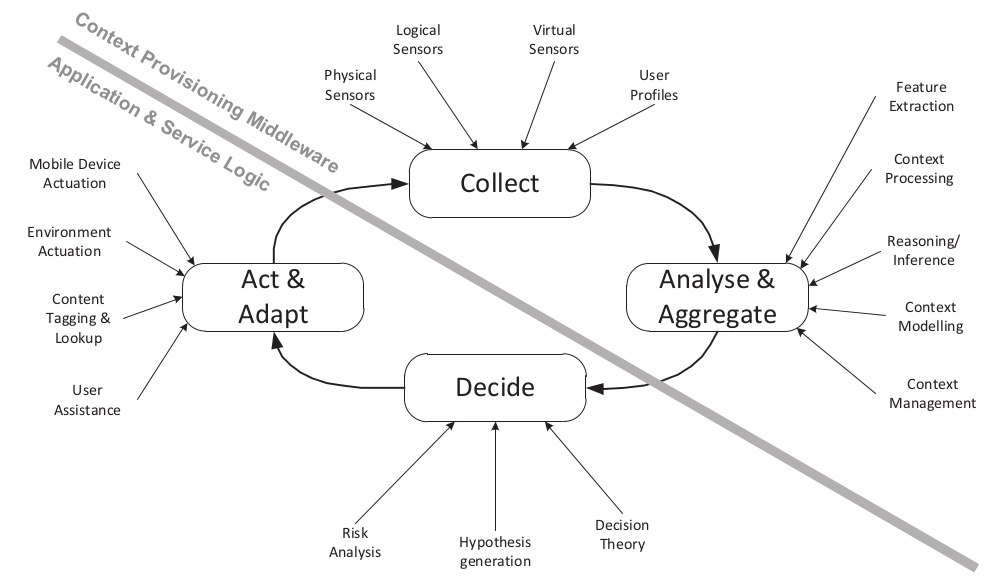
\includegraphics[width=0.5\linewidth]{figura3}}
\caption{The Context-Aware System Cycle (adapted from [12])}
\label{fig:speciation}
\end{figure}

%This article presents a retrospective view of the means by which existing context-aware systems carry out their functions using their constituent components for provision of contextual information and services. The comprehensive review and analyses provided in the following sections are focussed on how context-aware middleware systems undertake context modelling, management, provisioning and reasoning. Particularly, we analyse how such complex and interwoven systems, with the difficult task of bridging the virtual and real worlds, can be evaluated through multidisciplinary approaches.

Este artigo apresenta uma visão retrospectiva dos meios pelos quais os sistemas sensíveis ao contexto existentes exercem as suas funções com os seus elementos constitutivos para a prestação de serviços de informação e contextual. A revisão e análises previstas nas seguintes seções abrangentes são focado em como os sistemas de middleware context-aware realizar contexto de modelagem, gerenciamento, provisionamento e raciocínio. Particularmente, analisa-se como sistemas complexos e interligados, tais com a difícil tarefa de superar os mundos virtual e real, pode ser avaliada através de abordagens multidisciplinares.

%------------------------------------------------

\subsection{Major Contributions} % Sub-section

%This article assembles the state of the art in the multifarious aspects of context-aware systems. The comprehensive review and analyses of these aspects contains significant contributions in the following categories:

Este artigo reúne o estado da arte nos aspectos multiformes de sistemas sensíveis ao contexto. A ampla revisão e análise destes aspectos contém contribuições significativas nas seguintes categorias:

\begin{itemize}
%	\item The concept of context: Elaboration of the conceptual definition of context and context-awareness, including a view of how the definition of context has evolved over time, especially regarding human computer interaction.
	\item O conceito de contexto: Elaboração da definição conceitual do contexto e do contexto consciência, incluindo uma visão de como a definição do contexto tem evoluído ao longo do tempo, especialmente em relação a interação homem-computador.
%	\item Context modelling: A review of the context modelling and representation approaches, classifications of context models, the significance of context meta data and discussion on the features exposed by various context models that affect the utility and suitability of these models.
	\item Contexto de modelagem: A revisão da modelagem de contexto e abordagens, classificações de modelos de contexto, o significado de meta-dados de contexto e discussão 	sobre as características expostas por vários modelos de contexto que afetam a utilidade e adequação destes modelos de representação.
%	\item Context management: Identification of distinct functions carried out by context provisioning middleware and a review of existing classification of these systems. We present the basis of new classifications in terms of design, architecture and technology based parameters. A review of existing context provisioning middleware is presented, which serves as a basis for developing our novel three-tier classification based on the conceptual design model (layered, object-oriented, event-based, etc.) of a context provisioning middleware, the resulting architecture and implementation (central server, multiple-distributed servers, peer-to-peer, etc.) and an intersection of these two categories. Our classification presents a novel view for examining context provisioning middleware.
	\item Gerenciamento de contexto: Identificação de funções distintas realizadas pelo contexto provisionamento middleware e uma revisão da classificação existente desses sistemas. Nós apresentamos a base de novas classificações em termos de design, arquitetura e tecnologia parâmetros baseados. Uma análise do contexto provisionamento middleware existente é apresentada, que serve como base para o desenvolvimento de nosso novo classificação de três níveis com base no modelo de projeto conceitual (camadas, orientado a objetos, baseado em eventos, etc) de um middleware de provisionamento contexto, o resultando arquitetura e implementação (servidor central, servidores de múltipla distribuídos, peer-to-peer, etc) e uma interseção dessas duas categorias. Nossa classificação apresenta uma nova visão para o exame contexto provisionamento middleware.
%	\item Context reasoning: We discuss the role of context reasoning as a critical function provided by context provisioning middleware, highlight the variety of multi-disciplinary techniques employed in context provisioning middleware and review the most prominent of these techniques. The context reasoning and processing approaches are categorised with respect to their requirements and features, and examples of their application domains are provided as well.
	\item Contexto raciocínio: Discutimos o papel do raciocínio contexto como uma função crítica fornecida pelo contexto provisionamento middleware, destacar a variedade de técnicas multi-disciplinares empregadas no contexto provisionamento middleware e revise o mais proeminente destas técnicas. O raciocínio contexto e abordagens de processamento são categorizadas com relação às suas necessidades e características, e exemplos de seus domínios de aplicação são fornecidos também.
%	\item Evaluation of context middleware: A major contribution of this article is the detailed discussion on the evaluation strategies and mechanisms of context provisioning middleware. We identify the challenges faced in evaluating a multidisciplinary domain, review the approaches used in evaluation of contemporary context middleware as a whole and that of their individual functions and components, identify the recent trends and evolution of evaluation methodologies in these systems. A comparison of these evaluation methodologies, with respect to the target environment and requirements, is also presented along with examples from the state of the art.
	\item Avaliação do contexto middleware: A principal contribuição deste artigo é a discussão detalhada sobre as estratégias e os mecanismos de provisionamento contexto middleware avaliação. Nós identificamos os desafios enfrentados na avaliação de um domínio multidisciplinar, rever os métodos utilizados na avaliação de middleware contexto contemporâneo como um todo e de suas funções e componentes individuais, identificar as tendências recentes e evolução de metodologias de avaliação desses sistemas. Uma comparação destas metodologias de avaliação, em relação ao meio ambiente e requisitos alvo, também é apresentado, juntamente com exemplos do estado da arte.
%	\item Domain outlook: Finally, the domain of context provisioning is discussed in a broader perspective, highlighting the overlap and its interaction with other research disciplines. Based on lessons learnt and recent trends, we sketch the expected evolution and identify future research objectives.
	\item Domínio do Outlook: Finalmente, o domínio de provisionamento contexto é discutido em uma perspectiva mais ampla, com destaque para a sobreposição e sua interação com outras disciplinas. Com base nas lições aprendidas e tendências recentes, esboçar a evolução esperada e identificar futuros objetivos da pesquisa.
\end{itemize}

%Our objective is not only to present an in depth coverage of the approaches taken in fulfilling the critical functions of context provisioning middleware, but also to present a guide that comprehensively introduces the domain of context-aware systems to new researchers. To achieve this objective, it is essential to present the background and definitions of pertinent domain concepts, which we do so in Section II. The overall article structure is described in the following subsection.

Nosso objetivo não é apenas apresentar uma cobertura em profundidade das abordagens adotadas para cumprir as funções críticas do contexto provisionamento middleware, mas também para apresentar um guia abrangente que apresenta o domínio de sistemas sensíveis ao contexto para novos pesquisadores. Para atingir este objectivo, é essencial para apresentar o plano de fundo e definições de conceitos de domínio pertinentes, o que fazemos para que na Seção II. A estrutura geral do artigo é descrito na subsecção seguinte.

%------------------------------------------------

\subsection{Structure} % Sub-section

%We first of all elaborate the concepts of ubiquitous computing, context, and context-awareness as required background knowledge in Section II. Context modelling and representation are discussed from a classification perspective in Section III and the context management approaches adopted in existing systems are discussed and analysed in Section IV. Section V contains a discussion on the context reasoning and inference mechanisms. Section VI presents a detailed review and analysis on the evaluation techniques of these middleware systems. In this article decision taking is not covered, actuation and adaptation are only briefly addressed when discussing the evaluation (Section VI). The article finally concludes with a summary, presentation of future trends and discussion of open issues in Section VII.

Primeiro de tudo elaborado os conceitos de computação ubíqua, contexto e contexto consciência como conhecimento de fundo exigido na Seção II. Contexto de modelagem e representação são discutidos a partir de uma perspectiva de classificação na Seção III eo gerenciamento de contexto abordagens adoptadas nos sistemas existentes são discutidos e analisados ​​na Seção IV. Seção V contém uma discussão sobre o raciocínio contexto e mecanismos de inferência. Seção VI apresenta uma revisão detalhada e análise sobre as técnicas de avaliação desses sistemas de middleware. Neste artigo, a tomada de decisão não é coberto, atuação e adaptação são apenas abordadas brevemente quando se discute a avaliação (Seção VI). O artigo, finalmente, conclui com um resumo, apresentação de tendências futuras e discussão de questões abertas na Secção VII.


%----------------------------------------------------------------------------------------
%	CONCLUSÃO
%----------------------------------------------------------------------------------------

\section{Conclusão} % Major section

%This article has presented a comprehensive review and analysis of how context-aware middleware systems undertake context modelling, management, reasoning and provisioning related functions. By examining the state-of-the-art in the multifarious aspects of context-awareness, the article has aimed at developing an understanding of the functional diversity of the middleware bridging the virtual and real worlds. We have also examined how such complex and interwoven systems can be evaluated through multidisciplinary approaches. Based on the discussions and analyses of various domain specific topics, this article has also presented the main trends and ongoing evolution of context provisioning. Open research issues have been identified and recommended for future work.

Este artigo apresentou uma revisão abrangente e análise de como os sistemas de middleware sensíveis ao contexto comprometem contexto de modelagem, gerenciamento, raciocínio e provisionamento funções relacionadas. Ao examinar o state-of-the-art nos aspectos multiformes de contexto-consciência, o artigo teve como objetivo o desenvolvimento de uma compreensão da diversidade funcional do middleware ponte entre os mundos virtual e real. Examinamos, também, tais como os sistemas complexos e interligados pode ser avaliada através de abordagens multidisciplinares. Com base nas discussões e análises de vários temas de domínio específico, este artigo também apresentou as principais tendências e evolução contínua de fornecimento de contexto. Questões de pesquisa em aberto foram identificados e recomendados para o trabalho futuro.

%----------------------------------------------------------------------------------------
%	BIBLIOGRAPHY
%----------------------------------------------------------------------------------------

%\begin{thebibliography}{99} % Bibliography - this is intentionally simple in this template

%\bibitem[Figueredo and Wolf, 2009]{Figueredo:2009dg}
%Figueredo, A.~J. and Wolf, P. S.~A. (2009).
%\newblock Assortative pairing and life history strategy - a cross-cultural
%  study.
%\newblock {\em Human Nature}, 20:317--330.
 
%\end{thebibliography}

%----------------------------------------------------------------------------------------

\end{document}

